\chapter{Regression}
As hinted to before, a major problem that machine learning hopes to solve is being able to predict some target value $y$ given some explanatory inputs $x$. When this prediction is a continuous, real number, we call this prediction procedure \emph{regression}.

We can think of a few real-world situations where it would be helpful to be able to predict continuous targets:

\begin{enumerate}
    \item Predicting a person's height given the height of their parents.
    \item Predicting the amount of time someone will take to pay back a loan given their credit history.
    \item Predicting what time a package will arrive given current weather and traffic conditions.
\end{enumerate}

In each of these examples, we are trying to estimate a single value after being given one or more input values. The assumption is that these inputs hopefully encode enough information about the desired target value. It seems reasonable to predict a person's height given their parents' heights. However, it seems foolish to try to predict stock prices given meteorlogical activity on Mars. An attempt to do either of these is indeed still regression. The term ``regression'' is general and encompasses any method that will predict a value by trying to model its relationship to some inputs.

\begin{definition}[regression]
    A class of method that make predictions about unknown target $y$ given observed inputs $x$.
\end{definition}


% \section{Solution Options}
% Now that you understand the type of problems we are trying to solve with regression, we can start to think at a high level of the different ways we might arrive at a solution. Here is a short, nonexhaustive list of regression techniques with brief explanations:

% \subsection{$K$-Nearest neighbors}
% $K$-Nearest neighbors is an extremely intuitive, non-parametric technique for regression or classification. It works as follows in the regression case:

% \begin{itemize}
%     \item Identify the $K$ points in our dataset that are closest to the new data point. ``Closest'' is some measure of distance, usually Euclidean.
%     \item Average the value of interest for those $K$ data points.
%     \item Return that averaged value of interest: it is the prediction for our new data point.
% \end{itemize}

% \begin{warning}
%     A \textit{non-parametric} model simply means we don't make any assumptions about the form of our data. We only need to use the data itself to make predictions.
% \end{warning}

% \subsection{Neural networks}
% A neural network works by scaling and combining input variables many times. Furthermore, at each step of scaling and combining inputs, we typically apply some form of \textit{nonlinearity} over our data values. The proof is beyond the scope of this textbook, but neural networks are known to be \textit{universal function approximators}. This means that given enough scaling and combining steps, we can approximate any function to an arbitrarily high degree of accuracy using a neural network.

% \subsection{Random forests}
% Random forests are what's known as an \textit{ensemble method}. This means we average the results of many smaller regressors known as \textit{decision trees} to produce a prediction. These decision trees individually operate by partitioning our original dataset with respect to the value of predictive interest using a subset of the features present in that dataset. Each decision tree individually may not be a reliable regressor; by combining many of them we achieve a model with better performance.

% \subsection{Gradient boosted trees}
% Gradient boosted trees are another technique built on decision trees. Assume we start with a set of decision trees that together achieve a certain level of performance. Then, we iteratively add new trees to improve performance on the hardest examples in our dataset, and reweight our new set of decision trees to produce the best level of performance possible.

% \subsection{Turning to linear regression}
% You've likely never even heard of some of these preceding techniques - that's okay. The point is that we have a number of existing methods that take different approaches to solving regression problems. Each of these will have their own strengths and weaknesses that contribute to a decision about whether or not you might use them for a given regression problem. We obviously do not cover these methods in great detail here; what's more important is the understanding that there are a variety of ways to go about solving regression problems. From here on out, we will take a deeper dive into linear regression. There are several reasons for which we are exploring this specific technique in greater detail. The two main reasons are that it has been around for a long time and thus is very well understood, and it also will introduce many concepts and terms that will be utilized extensively in other machine learning topics.

\section{Linear Regression}
The simplest form of regression is \emph{linear regression}, which predicts the target value by taking a linear combination of the input features.

\begin{definition}[linear regression]
    Linear regression is the process of predicting the target value of some input features $\bm x \in \mathbb R^d$ through the linear function
    \begin{equation}
        \label{eq:linreg}
        f(\bm x; \bm w) := w_0 + w_1 x_1 + \ldots + w_d x_d.
    \end{equation}
\end{definition}

A linear regression model $f(\bm x; \bm w)$ is fully specified by its weights $\bm w$. Therefore, we refer to a model as simply the set of weights $\bm w$ which parametrize it.

Technically, \autoref{eq:linreg} is affine, not linear, because it includes a bias term. For convinience, we often use the ``bias trick'' to express the model as a linear function:
\begin{equation}
    \label{eq:bias trick}
    f(\bm x; \bm w) = \bm w\T \bm x.
\end{equation}
This is possible because we impose $x_0 = 1$ for all $\bm x \in \mathbb R^d$. More specifically, we apply the following transformation before feeding our inputs into our model: $$\bm x = \cvec{x_1\\\vdots\\x_d} \mapsto \cvec{1\\x_1\\\vdots\\x_d}.$$ With this trick, we recover our original definition \autoref{eq:linreg}:
\begin{align*}
    f(\bm x; \bm w) &= \bm w\T \bm x \\
    &= w_0 x_0 + w_1 x_1 + \ldots + w_d x_d \\
    &= w_0 \cdot 1 + w_1 x_1 + \ldots + w_d x_d \\
    &= w_0 + w_1 x_1 + \ldots + w_d x_d.
\end{align*}

\begin{warning}
    Even though this adds a dimension to the input space, we still say that $\bm x \in \mathbb R^d$ for convinience-sake. This means we also say $\bm w \in \mathbb R^d$.
\end{warning}

\begin{example}[predicting height]
    Assume we are working in a healthcare setting and the doctor gives us a linear regression model $$\bm w = \cvec{34 \\ 0.39 \\ 0.33}$$ predict any child's future height. The model assumes we represent any child $\bm x$ by two features: $x_1$ describing the mother's height (in cm) and $x_2$ describing the father's height (in cm). If the child's mother is 165cm tall and father 185cm tall, then $$\bm x^* = \cvec{165 \\ 185}$$ represents the child which we hope to make a prediction for. Using our model, we predict this child's future height is $$\hat y^* := f(\bm x^*; \bm w) = \bm w\T \bm x^* = 34 + 0.39(165) + 0.33(185) = 159.4.$$ Notice the use of $\hat y^*$ to mean our model prediction.
\end{example}

% Let's inspect the categories linear regression falls into for our ML framework cube:
% \begin{mlcube}[Non-Probabalistic Linear Regression]{Continuous}{Supervised}{No}
%  Linear regression deals with a continuous output space $\mathcal Y \in \mathbb R$. As we will explore soon, we learn which weights to use by looking at preexisting examples of ideal predictions. Using this labelled dataset in training makes regression a \textbf{supervised} technique. So far regression is \textbf{non-probabilistic}. Note that there also exist probabilistic interpretations of linear regression which we will discuss later in the chapter.
% \end{mlcube}

\subsection{Visualizing a linear regression model}
Let's try to build some intuition about how linear regression works. Our algorithm is given a labelled training dataset $\mathcal D = \{(\bm x_i, y_i)\}_{i=1}^{n}$ where $\bm x_i \in \mathbb R^d$ is the $i$-th input and $y_i \in \mathbb R$ is that input's corresponding target. Our goal is to find weights $\bm w$ such that given a new data point $\bm x^* \not \in \mathcal D$, we can predict its target value $y^*$. Admittedly, it is not likely that we can exactly predict the true target $y^*$ for every $\bm x \in \mathcal X$. (In fact, just the idea that there even exists a true $y^*$ out there is imposed by us). Hence, we instead try to estimate $y^*$ with a different but hopefully ``close" value $\hat y^*$ (we can define what close means in many ways). This is visualizable in the simple case where we only have 1-dimensional inputs: $\mathcal{X} \subset \mathbb{R}$.

\begin{figure}
    \centering
    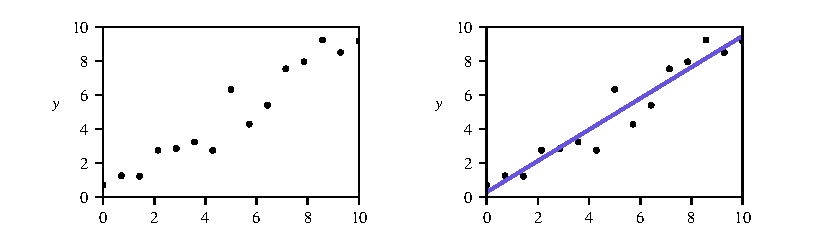
\includegraphics{simple-lin-reg}
    \caption{A dataset with a clear linear trend (left). A line which seems to fit the apparent linear relationship (right).}
    \label{fig:simple-lin-reg}
\end{figure}

Our eyes are naturally able to detect the very clear trend in this data. If we were given a datapoint $\bm x^*$, not necessarily in our training dataset, how would we predict its target value $y^*$? We would first fit a line to our data, as in \autoref{fig:simple-lin-reg} (right), and then we select $\hat y^*$ according to the point $(\bm x^*, \hat y^*)$ on the line.

That is the entirety of linear regression. It fits a line to our training data, and then uses that line to make predictions. In 1-dimensional input space, this manifests itself as the simple problem seen above,where  we need only find a single bias term $w_0$ (which acts as the intercept of the line) and single weight $w_1$ (which acts as the slope of the line). However, the same principle applies to higher dimensional data as well. We're always fitting the hyperplane that best predicts the data.

\begin{warning}
    Although our input data points $\bm x$ can take on multiple dimensions, our output data $y$ is always a 1-dimensional real number when dealing with regression problems.
\end{warning}


\subsection{Least squares loss}
% Now that we have some intuition for what linear regression is, a natural question arises: how do we find the optimal values for $\bm w$?
Now that we've defined our model as a weighted combination of our input variables, we need some way to choose our value of $\bm w$. To do this, we need an objective or loss function.

Recall that the objective function measures the ``goodness'' of a model. We can optimize this function to identify the best possible model for our data. Note that in the case of linear regression, our model is entirely specified by our settings of parameters $\bm w$.

An objective function will sometimes be referred to as \textit{loss}. Loss actually measures how bad a model is, and then our goal is to minimize it. It is common to think in terms of loss when discussing linear regression, and we incur loss when the hyperplane we fit is far away from our data.

So how do we compute the loss for a specific setting of $\bm w$? To do this, we often use \emph{residuals}.

\begin{definition}[residual]
    The residual is the difference between the target $y$ and prediction $\hat y = f(\bm x; \bm w)$ value that a model produces: $$y - f(\bm x; \bm w) = y - \bm w\T \bm x.$$
\end{definition}

Commonly, loss is a function of the residuals produced by a model. For example, you can imagine taking the absolute value of all of the residuals and adding those up to produce a measurement of loss. This is referred to as \textit{L1 loss}. Or, you might square all of the residuals and then add those up to produce loss, which is called \textit{L2 loss} or \textit{least squares loss}. You might also use some combination of L1 and L2 loss. For the most part, these are the two most common forms of loss you will see when discussing linear regression.

\begin{definition}[least squares loss]
    The least squares loss of a model $\bm w$ over a labelled dataset $\mathcal D$ is the sum of the squared residuals or ``losses'': $$\mathcal L(\bm w; \mathcal D) := \frac12 \sum_{(\bm x, y) \in \mathcal D} (y - f(\bm x; \bm w))^2.$$
\end{definition}

\begin{warning}
    Notice that our summation happens over the dataset: this means that for same model $\bm w$ can have very different losses depending on the training dataset collected. This is why we hope our training dataset is an accurate representation of the entire global dataset of possible inputs yet seen. We often will leave this out as implicit, simply using $\mathcal L(\bm w)$.
\end{warning}

When minimized, these distinct measurements of loss will produce solutions for $\bm w$ that have different properties. For example, L2 loss is not robust to outliers due to the fact that we are squaring residuals. Furthermore, L2 loss will produce only a single solution while L1 loss can potentially have many equivalent solutions. Finally, L1 loss produces unstable solutions, meaning that for small changes in our dataset, we may see large changes in our solution $\bm{w}$.

Loss is a concept that we will come back to very frequently in the context of supervised machine learning methods. Before exploring exactly how we use loss to fit a line, let's consider least squares loss in greater depth.


There is a satisfying statistical interpretation for using this loss function which we will explain later in this chapter, but for now it will suffice to discuss some of the properties of this loss function that make it desirable.

First, notice that it will always take on positive values. This is convenient because we can focus exclusively on minimizing our loss, and it also allows us to combine the loss incurred from different data points without worrying about them cancelling out.

A more subtle but enormously important property of this loss function is that it is strongly convex. This means we also know that there exists a unique global minimum where the derivative of the function is equal to 0, as seen in \autoref{fig:lin-reg-minima}. This is in part credit to the fact that strongly convex functions are continuously differentiable. In contrast, L1 loss is not continuously differentiable over the entirety of its domain.

\begin{figure}
    \centering
    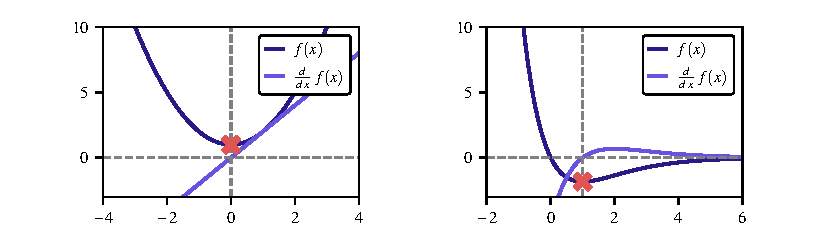
\includegraphics{lin-reg-minima}
    \caption{Strongly convex functions are minimized where their derivative 0.}
    \label{fig:lin-reg-minima}
\end{figure}

\subsection{Solving for Optimal Weights Analytically}
Now that we have our least squares loss function, we can finally begin to fit a line to our data. Our goal is to find the optimal set of weights $\bm{w}^*$ with respect to a particular labelled training dataset $\mathcal{D}$: $$\bm{w}^* := \argmin_w \mathcal{L}(\bm{w}; \mathcal{D}).$$

For convinience, we can concatenate our dataset $\mathcal{D} := \{(\bm{x}_i, y_i)\}_{i=1}^{n}$ as $\mathcal{D} = (\bm{X}, \bm{y})$ where $\bm{X} := [\bm{x}_1, \ldots, \bm{x}_n]\T \in \mathbb{R}^{n \times d}$ and $\bm{y} := [y_1, \ldots, y_n]\T$. The matrix $\bm{X}$ is commonly referred to as the \emph{design matrix}.

\begin{derivation}[least squares optimal weights]
    \label{der:least-squares-derivation}
    We find the optimal weights $\bm{w}^*$ as follows:

    Start by taking the gradient of the loss with respect to our parameter $\bm{w}$: $$\nabla \mathcal{L}(\bm{w}; \mathcal D) = \sum_{n=1}^{N} (y_n - \bm{w}\T \bm{x}_n)(-\bm{x}_n).$$

    Setting this gradient to 0 and multiplying both sides by -1, we get 
    \begin{align*}
        0 &= \sum_{n=1}^{N} y_n \bm{x}_n - \sum_{n=1}^N (\bm{w}\T\bm{x}_n)\bm{x}_n \\
        &= \sum_{n=1}^{N} y_n \bm{x}_n - \sum_{n=1}^N \bm{x}_n(\bm{x}_n\T\bm{w}).
    \end{align*}
    
    We get this last line by noticing that $(\bm{w}\T\bm{x}_n)\bm{x}_n = (\bm{x}_n\T\bm{w})\bm{x}_n = \bm{x}_n(\bm{x}_n\T\bm{w})$. (This is because $a\T=a$ and $a\bm{v}=\bm{v}a$ for any scalar $a$ and vector $\bm{v}$).

    At this point, it is convenient to rewrite these summations as matrix operations. Using the design matrix $\bm{X}$ and target values $\bm{y}$, we have
    \begin{align*}
    \bm{X}\T\bm{y}=\sum_{n=1}^N y_n \bm{x}_n, \quad
    \bm{X}\T\bm{X}\bm{w}=\sum_{n=1}^N\bm{x}_n(\bm{x}_n\T\bm{w}).
    \end{align*}

    After substituting, $$0 = \bm{X}\T\bm{y} - \bm{X}\T\bm{X}\bm{w},$$

    we can solve for $\bm{w}^*$:
    \begin{equation}
        \label{eq:least-squares-solved-for-w}
        \bm{w}^* = (\bm{X}\T \bm{X})^{-1} \bm{X}\T \bm{y}.
    \end{equation}

    For this to be well defined we need $\bm{X}$ to have full column rank (features are not colinear) so that $\bm{X}\T \bm{X}$ is positive definite and the inverse exists.
\end{derivation}

The quantity $(\bm{X}\T\bm{X})^{-1}\bm{X}\T$ in \autoref{der:least-squares-derivation} has a special name: the \emph{Moore-Penrose pseudoinverse}. You can think of it as the generalization of matrix inversion for non-square matrices.

\subsection{Solving for Optimal Weights Geometrically}
Another common interpretation of linear regression is that of a projection of our targets, $\bm{y}$, onto the column space of our inputs $\bm{X}$. This can be useful for building intuition.

We showed above that the quantity $(\bm{X}\T\bm{X})^{-1}\bm{X}\T$ can be thought of as the pseudoinverse for our inputs $\bm{X}$. Let's now consider the case where $\bm{X}$ is square and the pseudoinverse is equal to the true inverse: $\bm{X}^{-1} = (\bm{X}\T\bm{X})^{-1}\bm{X}\T$. With this assumption,
\begin{align*}
    \bm{w}^* &= (\bm{X}\T\bm{X})^{-1}\bm{X}\T\bm{y} \\
    &= \bm{X}^{-1}\bm{y}.
\end{align*}

We can recover our target values $\bm{y}$ by multiplying either side by $\bm{X}$:
\begin{align*}
    \bm{X}\bm{w}^* &= \bm{X}\bm{X}^{-1}\bm{y} \\
    \bm{X}\bm{w}^* &= \bm{y}
\end{align*}

We were able to recover our targets $\bm{y}$ exactly because $\bm{X}$ is an invertible tranformation. However, in the general case where $\bm{X}$ is not invertible and we have to use the approximate pseudoinverse $(\bm{X}\T\bm{X})^{-1}\bm{X}\T$, we instead recover $\hat{\bm{y}}$:
\begin{align*}
    \bm{X}\bm{w}^* = \bm{X}(\bm{X}\T\bm{X})^{-1}\bm{X}\T\bm{y} \\
    \bm{X}\bm{w}^* = \hat{\bm{y}}
\end{align*}
where $\hat{\bm{y}}$ can be thought of as the closest projection of $\bm{y}$ onto the column space of $\bm{X}$.

This motivates the intuition that $\bm{w}^*$ is the set of coefficients that best transforms our input space $\bm{X}$ into our target values $\bm{y}$.

\section{Probabalistic Linear Regression}
We've thus far been discussing linear regression exclusively in terms of a loss function that helps us fit a set of weights to our data. In particular, we have been working with least squares, which has nice properties that make it a reasonable loss function.

In a very satisfying fashion, least squares also has a statistical foundation. In fact, you can recover the least squares loss function purely from a statistical derivation that we present here.

Consider our dataset $\mathcal D = \{(\bm x_i, y_i)\}_{i = 1}^{n}$, where $\bm{x}_n \in\mathbb R^d$ and $y \in\mathbb{R}$. Let's imagine that every label $y_i$ was generated from a probability distribution determined by $\bm x_i$ in some way. Namely, imagine $y_i$ is a realization of the random variable
\begin{align*}
    \mathrm y_i \sim \mathcal{N}(\bm w\T \bm x_n, \sigma^2).
\end{align*}
The PDF of the r.v. $\mathrm y_i$ is hence given by:
\begin{equation}
    \label{eq:normal-over-w}
    P(\mathrm y_i = y_i) = p(y_i; \bm x_i, \bm w) = \mathcal{N}(y_i; \bm w\T \bm x_i, \sigma^2)
\end{equation}

The interpretation of the story we are imposing here is that each datapoint's label is drawn randomly. This story makes sense: if a doctor measures a patient's blood pressure, there is randomness associated with the imperfections of the instruments with which the measurements were taken. By assuming each label $\mathrm y_i$ is distributed as Gaussian with mean $\bm w\T \bm x_i$, we are assuming that it is unlikely to see $y_i$ far from $\bm w\T \bm x_i$.

Also notice that $\sigma^2$ is fixed. Namely, $p(y_i; \bm x_i, \bm w)$ is not parametrized by $\sigma^2$. It absolutely can be. In fact, we can assume a different variance for every single training datapoint. But, assuming they all have the same variance is a common and safe assumption (and we will see why).

\begin{warning}
    Notice the notational difference between the r.v. $\mathrm y$ (normal case) and the realization $y$ (italics). Also notice the difference between $\mathcal{N}(\mu, \sigma^2)$, the Gaussian distribution with mean $\mu$ and variance $\sigma^2$, and its the PDF $$\mathcal{N}(x; \mu, \sigma^2) := \frac{1}{\sqrt{2 \pi \sigma^2}} \exp\left( -\frac12 \frac{(x-\mu)^2}{\sigma^2} \right).$$
\end{warning}

\subsection{Maximum likelihood estimation}

As before, how do we solve for the optimal weights $\bm w$? One approach we can take is to choose the weights $\bm w$ which maximize the likelihood of observing our labels $\bm y$. This technique is known as \textit{maximum likelihood estimation}.

The likelihood of some weights $\bm{w}$ is the probability of observing our $\mathcal D := (\bm{X}, \bm{y})$ given those weights: $$\ell(\bm{w}; \mathcal D) := \prod_{i=1}^n p(y_i; \bm{x}_i, \bm{w}).$$ Since we assume the training datapoints are independent, we simply multiplied the probabilities $P(\mathrm y_i = y_i)$ together. Our goal is to find the optimal model $\bm{w}^*$ which maximizes the likelihood of our training data: $$\bm{w}^* := \argmax_{\bm{w}} \ell(\bm{w}; \mathcal D).$$

\begin{derivation}[MLE optimal weights]
    The likelihood of our model $\bm{w}$ given a dataset $\mathcal D = (\bm{X}, \bm{y})$ and a fixed variance $\sigma^2$ is given by
    \begin{align*}
        p(\bm{y} \mid \bm{X}, \bm{w}, \beta) = \prod_{n=1}^{N} \mathcal{N}(\bm{w}\T\bm{x}_n, \beta^{-1})
    \end{align*}
    We then take the logarithm of the likelihood, and since the logarithm is a strictly increasing, continuous function, this will not change our optimal weights $\bm{w}$:
    \begin{align*}
        \ln{p(\bm{y} \mid \bm{X}, \bm{w}, \beta)} = \sum_{n=1}^{N} \ln{\mathcal{N}(\bm{w}\T\bm{x}_n, \beta^{-1})}
    \end{align*}
    Using the density function of a univariate Gaussian:
    \begin{align*}
        \ln{p(\bm{y} \mid \bm{X}, \bm{w}, \beta)} &= \sum_{n=1}^{N} \ln{\frac{1}{\sqrt{2\pi\beta^{-1}}} e^{-(y_n - \bm{w}\T\bm{x}_n)^2 / 2\beta^{-1}}} \\
        &= \frac{N}{2}\ln{\beta} - \frac{N}{2}\ln{(2\pi)} - \frac{\beta}{2} \sum_{n=1}^{N} (y_n - \bm{w}\T\bm{x}_n)^2
    \end{align*}

    Notice that this is a quadratic function in $\bm{w}$, which means that we can solve for it by taking the derivative with respect to $\bm{w}$, setting that expression to 0, and solving for $\bm{w}$:
    \begin{align*}
      \frac{\partial \ln{p(\bm{y} | \bm{X}, \bm{w}, \beta)}}{\partial \bm{w}} & = -  \beta \sum_{n=1}^{N} (y_n - \bm{w}\T\bm{x}_n)(-\bm{x}_n)
      \\
      \Leftrightarrow \quad & 
      \sum_{n=1}^{N} y_n \bm{x}_n - \sum_{n=1}^N (\bm{w}\T\bm{x}_n)\bm{x}_n=0.
    \end{align*}

    Notice that this is exactly the same form as Equation \ref{least-squares-solving-for-w}. Solving for $\bm{w}$ as before, we have:
    \begin{equation}
        \label{eq:mle-solved-for-w}
        \bm{w}^* = (\bm{X}\T\bm{X})^{-1}\bm{X}\T\bm{y}
    \end{equation}
\end{derivation}

Notice that our final solution is exactly the same form as the solution in \autoref{eq:least-squares-solved-for-w}, which we solved for by minimizing the least squares loss! The takeaway here is that minimizing a least squares loss function is equivalent to maximizing the probability under the assumption of a linear model with Gaussian noise.

\section{Kernel Regression}
Occasionally, linear regression will fail to recover a good solution for a dataset. While this may be because our data doesn't actually have predictive power, it might also just indicate that our data is provided in a format unsuitable for linear regression. This section explores that problem, in particular focusing on how we can manipulate the flexibility of our models to make them perform better.

\subsection{Basis Functions}
There are some situations where linear regression is not the best choice of model for our input data $\bm{X}$. Because linear regression only scales and combines input variables, it is unable to apply more complex transformations to our data such as a \textit{sin} or square root function. In those situations where we need to transform our input variable somehow prior to performing linear regression (which is known as moving our data into a new \textit{basis}), we can apply a \textbf{basis function}.

\begin{definition}[basis function]
    Typically denoted by the symbol $\phi(\cdot)$, a basis function is a transformation applied to an input data point $\bm{x}$ to move our data into a different \textit{input basis}, which is another phrase for \textit{input domain}. \\

    For example, consider our original data point:
    \begin{align*}
    \bm{x} = (x^{(1)}, x^{(2)})'
    \end{align*}
    We may choose our basis function $\phi(\bm{x})$ such that our transformed data point in its new basis is:
    \begin{align*}
        \phi(\bm{x}) = (x^{(1)}, {x^{(1)}}^2, x^{(2)}, \sin(x^{(2)}))'
    \end{align*}

    Using a basis function is so common that we will sometimes describe our input data points as $\boldsymbol{\phi} = (\phi^{(1)}, \phi^{(2)}, ..., \phi^{(D)})'$.
\end{definition}

\begin{warning}
    The notation $\bm{x} = (x^{(1)}, x^{(2)})'$ is a way to describe the dimensions of a single data point $\bm{x}$. The term $\bm{x}^{(1)}$ is the first dimension of a data point $\bm{x}$, while $\bm{x}_1$ is the first data point in a dataset.
\end{warning}

Basis functions are very general - they could specify that we just keep our input data the same. As a result, it's common to rewrite the least squares loss function from Equation \ref{least-squares-loss-fn} for linear regression in terms of the basis function applied to our input data:

\begin{equation} \label{least-squares-loss-fn-w-basis}
    \mathcal{L}(\bm{w}) = \frac{1}{2} \sum_{n=1}^{N} (y_n - \bm{w}\T\boldsymbol{\phi}_n)^2
\end{equation}

To motivate why we might need basis functions for performing linear regression, let's consider this graph of 1-dimensional inputs $\bm{X}$ along with their target outputs $\bm{y}$, presented in Figure \ref{fig:lin-reg-no-basis-fn}.

\begin{figure}
    \centering
    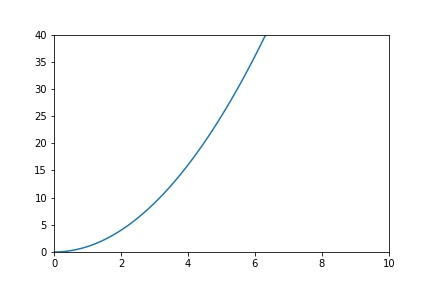
\includegraphics[width=0.5\paperwidth]{old/lin_reg_no_basis_fn_GEN.jpg}
    \caption{Data with no basis function applied.}
    \label{fig:lin-reg-no-basis-fn}
\end{figure}

As we can see, we're not going to be able to fit a good line to this data. The best we can hope to do is something like that of Figure \ref{fig:lin-reg-no-basis-fn-fitted}.

\begin{figure}
    \centering
    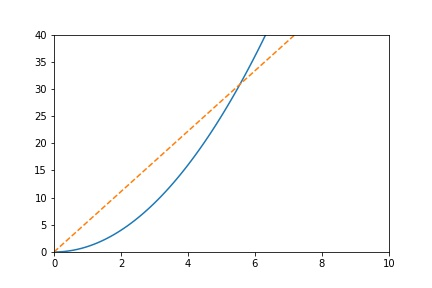
\includegraphics[width=0.5\paperwidth]{old/lin_reg_no_basis_fn_fitted_GEN.jpg}
    \caption{Data with no basis function applied, attempt to fit a line.}
    \label{fig:lin-reg-no-basis-fn-fitted}
\end{figure}

However, if we just apply a simple basis function to our data, in this case the square root function, $\phi(\bm{x}) = (\sqrt{x_1})'$, we then have the red line in Figure \ref{fig:lin-reg-w-basis-fn-fitted}. We now see that we can fit a very good line to our data, thanks to basis functions.

\begin{figure}
    \centering
    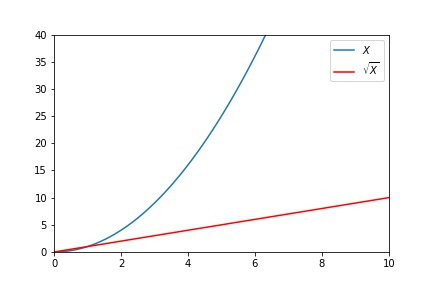
\includegraphics[width=0.5\paperwidth]{old/lin_reg_w_basis_fn_GEN.jpg}
    \caption{Data with square root basis function applied.}
    \label{fig:lin-reg-w-basis-fn-fitted}
\end{figure}

Still, the logical question remains: how can I choose the appropriate basis function? This toy example had a very obviously good basis function, but in general with high-dimensional, messy input data, how do we choose the basis function we need?

The answer is that this is not an easy problem to solve. Often, you may have some domain specific knowledge that tells you to try a certain basis, such as if you're working with chemical data and know that an important equation involves a certain function of one of your inputs. However, more often than not we won't have this expert knowledge either. Later, in the chapter on neural networks, we will discuss methods for discovering the best basis functions for our data automatically.

\subsection{Regularization}
When we introduced the idea of basis functions above, you might have wondered why we didn't just try adding many basis transformations to our input data to find a good transformation. For example, we might use this large basis function on a $D$-dimensional data point $\bm{z}$:
\begin{align*}
    \phi(\bm{z}) = (z^{(1)}, {z^{(1)}}^{2}, ..., {z^{(1)}}^{100}, z^{(2)}, {z^{(2)}}^{2}, ..., {z^{(2)}}^{100}, ..., z^{(D)}, {z^{(D)}}^{2}, ..., {z^{(D)}}^{100})'
\end{align*}
where you can see that we expand the dimensions of the data point to be 100 times its original size.

Let's say we have an input data point $\bm{x}$ that is 1-dimensional, and we apply the basis function described above, so that after the transformation each data point is represented by 100 values. Say we have 100 data points on which to perform linear regression, and because our transformed input space has 100 values, we have 100 parameters to fit. In this case, with one parameter per data point, it's possible for us to fit our regression line perfectly to our data so that we have no loss! But is this a desirable outcome? The answer is no, and we'll provide a visual example to illustrate that.

Imagine Figure \ref{fig:data-set-scattered} is our dataset. There is a very clear trend in this data, and you would likely draw a line that looks something like that of Figure \ref{fig:data-set-natural-fit} to fit it.

\begin{figure}
    \centering
    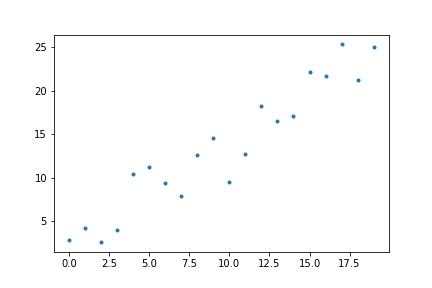
\includegraphics[width=0.5\paperwidth]{old/data_set_scattered_GEN.jpg}
    \caption{Dataset with a clear trend and Gaussian noise.}
    \label{fig:data-set-scattered}
\end{figure}

\begin{figure}
    \centering
    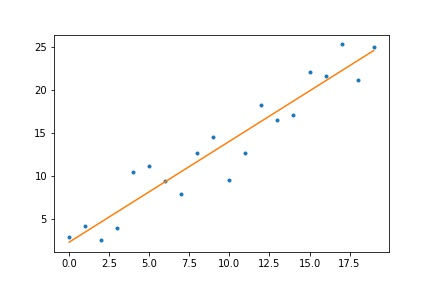
\includegraphics[width=0.5\paperwidth]{old/data_set_natural_fit_GEN.jpg}
    \caption{Natural fit for this dataset.}
    \label{fig:data-set-natural-fit}
\end{figure}

However, imagine we performed a large basis transformation like the one described above. If we do that, it's possible for us to fit our line perfectly, threading every data point, like that in Figure \ref{fig:data-set-unnatural-fit}.

\begin{figure}
    \centering
    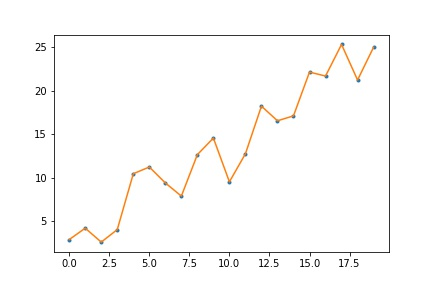
\includegraphics[width=0.5\paperwidth]{old/data_set_unnatural_fit_GEN.jpg}
    \caption{Unnatural fit for this dataset.}
    \label{fig:data-set-unnatural-fit}
\end{figure}

Let's see how both of these would perform on new data points. With our first regression line, if we have a new data point $\bm{x} = (10)'$, we would predict a target value of $\bm{14.1}$, which most people would agree is a pretty good measurement. However, with the second regression line, we would predict a value of $\bm{9.5}$, which most people would agree does not describe the general trend in the data. So how can we handle this problem elegantly?

Examining our loss function, we see that right now we're only penalizing predictions that are not correct in training. However, what we ultimately care about is doing well on new data points, not just our training set. This leads us to the idea of \textbf{generalization}.

\begin{definition}[generalization]
    Generalization is the ability of a model to perform well on new data points outside of the training set.
\end{definition}

A convoluted line that matches the noise of our training set exactly isn't going to generalize well to new data points that don't look exactly like those found in our training set. If wish to avoid recovering a convoluted line as our solution, we should also penalize the total size of our weights $\bm{w}$. The effect of this is to discourage many complex weight values that produce a messy regression line. By penalizing large weights, we favor simple regression lines like the one in Figure \ref{fig:data-set-natural-fit} that take advantage of only the most important basis functions.

The concept that we are introducing, penalizing large weights, is an example of what's known as \textbf{regularization}, and it's one that we will see come up often in different machine learning methods.

\begin{definition}[regularization]
    Applying penalties to parameters of a model.
\end{definition}

There is obviously a tradeoff between how aggressively we regularize our weights and how tightly our solution fits to our data, and we will formalize this tradeoff in the next section. However, for now, we will simply introduce a regularization parameter $\lambda$ to our least squares loss function:

\begin{equation} \label{least-squares-loss-fn-w-regularization}
    \mathcal{L}(\bm{w}) = \frac{1}{2} \sum_{n=1}^{N} (y_n - \bm{w}\T\boldsymbol{\phi}_n)^2 + \frac{\lambda}{2}\bm{w}^{\top}\bm{w}
\end{equation}

The effect of $\lambda$ is to penalize large weight parameters. The larger $\lambda$ is, the more we will favor simple solutions. In the limit $\lim_{\lambda\to\infty} \mathcal{L}(\bm{w})$, we will drive all weights to 0, while with a nonexistant $\lambda = 0$ we will apply no regularization at all. Notice that we're squaring our weight parameters - this is known as \textit{L2 norm regularization} or \textbf{ridge regression}. While L2 norm regularization is very common, it is just one example of many ways we can perform regularization.

To build some intuition about the effect of this regularization parameter, examine Figure \ref{fig:ridge-reg-diff-values}. Notice how larger values of $\lambda$ produce less complex lines, which is the result of applying more regularization. This is very nice for the problem we started with - needing a way to choose which basis functions we wanted to use. With regularization, we can select many basis functions, and then allow regularization to `prune' the ones that aren't meaningful (by driving their weight parameters to 0). While this doesn't mean that we should use as many basis transformations as possible (there will be computational overhead for doing this), it does allow us to create a much more flexible linear regression model without creating a convoluted regression line.

\begin{figure}
    \centering
    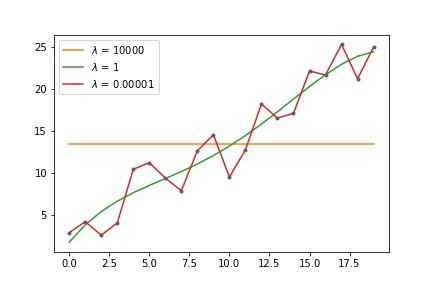
\includegraphics[width=0.5\paperwidth]{old/diffregvalues_GEN.jpg}
    \caption{Effect of different regularization parameter values on final regression solution.}
    \label{fig:ridge-reg-diff-values}
\end{figure}

\subsection{Generalizing Regularization}
We've thus far only discussed one form of regularization: ridge regression. Remember that under ridge regression, the loss function takes the form:
\begin{align*}
    \mathcal{L}(\bm{w}) = \frac{1}{2} \sum_{n=1}^{N} (y_n - \bm{w}\T\boldsymbol{\phi}_n)^2 + \frac{\lambda}{2}\bm{w}^{\top}\bm{w},
\end{align*}
%
where the $(\lambda/2)\bm{w}\T\bm{w}$ term is for the regularization. We can generalize our type of regularization by writing it as:
\begin{align*}
    \mathcal{L}(\bm{w}) = \frac{1}{2} \sum_{n=1}^{N} (y_n - \bm{w}\T\boldsymbol{\phi}_n)^2 + \frac{\lambda}{2}\big|\big|\bm{w}\big|\big|_h^{h}
\end{align*}
where $h$ determines the type of regularization we are using and thus the form of the optimal solution that we recover. For example, if $h=2$ then we add $\lambda/2$ times the square of the L2 norm.
%x
The three most commonly used forms of regularization are lasso, ridge, and elastic net. \newline \newline
\textbf{Ridge Regression} \newline
This is the case of $h = 2$, which we've already discussed, but what type of solutions does it tend to recover? Ridge regression prevents any individual weight from growing too large, providing us with solutions that are generally moderate. \newline \newline
\textbf{Lasso Regression} \newline
Lasso regression is the case of $h = 1$. Unlike ridge regression, lasso regression will drive some parameters $w_i$ to zero if they aren't informative for our final solution. Thus, lasso regression is good if you wish to recover a sparse solution that will allow you to throw out some of your basis functions. You can see the forms of ridge and lasso regression functions in Figure \ref{fig:ridge-and-lasso-reg-fn-form}.
If you think about how Lasso is L1 Norm (absolute value) and Ridge is L2 Norm (squared distance), you can think of those shapes as being the set of points $(w_1,w_2)$ for which the norm takes on a constant value.
%Just like a circle is a set of points at constant radius from its center, a rotated square with its vertices at [1,0], [-1,0], [0,1], [0,-1] is the set of 2D points with sum of abs values equal to 1.  
%
\newline
\newline

\textbf{Elastic Net} \newline
Elastic net is a middle ground between ridge and lasso regression, which it achieves by using a linear combination of the previous two regularization terms. Depending on how heavily each regularization term is weighted, this can produce results on a spectrum between lasso and ridge regression. \\

\begin{figure}
    \centering
    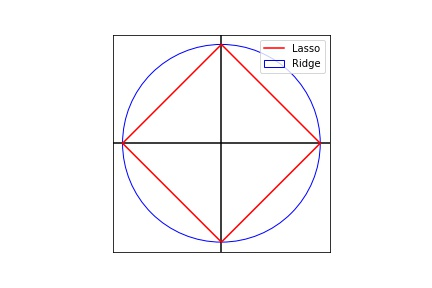
\includegraphics[width=0.5\paperwidth]{old/ridgeandlassoreg_GEN.jpg}
    \caption{Form of the ridge (blue) and lasso (red) regression functions.}
    \label{fig:ridge-and-lasso-reg-fn-form}
\end{figure}


\subsection{Bayesian Regularization} \label{bayesian-regularization-section}
We've seen regularization in the context of loss functions, where the goal is to penalize large weight values. How does the concept of regularization apply to Bayesian linear regression?

The answer is that we can interpret regularizing our weight parameters as adding a prior distribution over $\bm{w}$. Note that this is a different conception of regularization than we saw in the previous section. In the Bayesian framework, we are averaging over different models specified by different values of $\bm{w}$. Therefore, in this context regularization entails weighting models with smaller values of $\bm{w}$ more heavily.

\begin{derivation}[Bayesian Regularization Derivation]
    Because we wish to shrink our weight values toward 0 (which is exactly what regularization does), we will select a Normal prior with mean 0 and variance $\boldsymbol{S}_0^{-1}$:
    \begin{align*}
        \bm{w} \sim \mathcal{N}(0, \boldsymbol{S}_0^{-1}\bm{I})
    \end{align*}
    Remember from Equation \ref{normal-over-w} that the distribution over our observed data is Normal as well, written here in terms of our entire dataset:
    \begin{align*}
        p(\bm{y} | \bm{X}, \bm{w}, \beta) = \mathcal{N}(\bm{X}\bm{w}, \beta^{-1}\bm{I})
    \end{align*}
    % We want to combine the likelihood and the prior to recover the posterior distribution of $\bm{w}$, which follows directly from Bayes' Theorem:
    \begin{align*}
        \underbrace{p(\bm{w}|\bm{X},\bm{y}, \beta)}_{\text{posterior}} \propto \underbrace{p(\bm{y}| \bm{X}, \bm{w}, \beta)}_{\text{likelihood}}\underbrace{p(\bm{w})}_{\text{prior}}
    \end{align*}
    We now wish to find the value of $\bm{w}$ that maximizes the posterior distribution. We can maximize the log of the posterior with respect to $\bm{w}$, which simplifies the problem slightly:
    \begin{align*}
        \ln{p(\bm{w}|\bm{X},\bm{y}, \beta)} \propto \ln{p(\bm{y}| \bm{X}, \bm{w}, \beta)} + \ln{p(\bm{w})}
    \end{align*}
    Let's handle $\ln{p(\bm{y}| \bm{X}, \bm{w}, \beta)}$ first:
    \begin{align*}
        \ln{p(\bm{y}| \bm{X}, \bm{w}, \beta)} &= \ln{\prod_{n=1}^{N} \mathcal{N}(y_n | \bm{w}\T \bm{x}_n, \beta^{-1})} \\
        &= \ln{\prod_{n=1}^{N} \frac{1}{\sqrt{2\pi\beta^{-1}}} \exp{\bigg\{-\frac{\beta}{2}(y_n - \bm{w}\T \bm{x}_n)^2\bigg\}}} \\
        &= \bm{C} -\frac{\beta}{2}\sum_{n=1}^{N} (y_n - \bm{w}\T \bm{x}_n)^2 + \frac{1}{\sqrt{2\pi\beta^{-1}}}
    \end{align*}
    where $\bm{C}$ collects the constant terms that don't depend on $\bm{w}$. Let's now handle $\ln{p(\bm{w})}$:
    \begin{align*}
        \ln{p(\bm{w})} &= \ln{\mathcal{N}(0, \boldsymbol{S}_0^{-1}\bm{I})} \\
        &= \ln{\frac{1}{(|2\pi\boldsymbol{S}_0^{-1}\bm{I}|)^{\frac{1}{2}}} \exp{\bigg\{-\frac{\boldsymbol{S}_0}{2} \bm{w}\T\bm{w}\bigg\}}} \\
        &= \bm{C} -\frac{\boldsymbol{S}_0}{2} \bm{w}\T\bm{w}
    \end{align*}
    combining the terms for $\ln{p(\bm{y}| \bm{X}, \bm{w}, \beta)}$ and $\ln{p(\bm{w})}$:
    \begin{align*}
        \ln{p(\bm{w}|\bm{X},\bm{y}, \beta)} = -\frac{\beta}{2}\sum_{n=1}^{N} (y_n - \bm{w}\T \bm{x}_n)^2 - \frac{\boldsymbol{S}_0}{2} \bm{w}\T\bm{w}
    \end{align*}
    dividing by a positive constant $\beta$:
    \begin{align*}
        \ln{p(\bm{w}|\bm{X},\bm{y}, \beta)} = -\frac{1}{2}\sum_{n=1}^{N} (y_n - \bm{w}\T \bm{x}_n)^2 - \frac{\boldsymbol{S}_0}{\beta}\frac{1}{2} \bm{w}\T\bm{w}
    \end{align*}
    Notice that maximizing the posterior probability is equivalent to minimizing the sum of squared errors $(y_n - \bm{w}\T \bm{x}_n)^2$ and the regularization term $\bm{w}\T\bm{w}$.
\end{derivation}

\textbf{The interpretation of this is that adding a prior over the distribution of our weight parameters $\bm{w}$ and then maximizing the resulting posterior distribution is equivalent to adding a regularization term where $\lambda = \frac{\boldsymbol{S}_0}{\beta}$}

\section{Model Selection}
\subsection{Bias-Variance Tradeoff and Decomposition}
Now that you know about regularization, you might have some intuition for why we need to find a balance between complex and simple regression solutions. A complex solution, while it might fit all of our training data, may not generalize well to future data points. On the other hand, a line that is too simple might not vary enough to provide good predictions at all. This phenomenon is not unique to linear regression- it's actually a very fundamental concept in machine learning that's known as the \textbf{bias-variance tradeoff}.

\begin{definition}[Bias-Variance Tradeoff]
    When constructing machine learning models, we have a choice somewhere on a spectrum between two extremes: fitting exactly to our training data or not varying in response to our training data at all. The first extreme, fitting all of our training data, is a situation of high \textit{variance}, because our output changes heavily in reponse to our input data (see the red line in Figure \ref{fig:ridge-reg-diff-values}). At the other extreme, a solution that doesn't change in response to our training data at all is a situation of high \textit{bias} (see the yellow line in Figure \ref{fig:ridge-reg-diff-values}). This means our model heavily favors a specific form regardless of the training data, so our target outputs don't fluctuate between distinct training sets.
\end{definition}

Obviously a good solution will fall somewhere in between these two extremes of high variance and high bias. Indeed, we have techniques like regularization to help us balance the two extremes (improving generalization), and we have other techniques like \textit{cross-validation} that help us determine when we have found a good balance (measuring generalization).

\begin{warning}
    In case you are not familiar with the terms \textit{bias} and \textit{variance}, we provide their statistical definitions here:
    \begin{align*}
        \text{bias($\theta$)} = \mathrm{E}[\theta] - \theta
    \end{align*}
    \begin{align*}
        \text{variance($\theta$)} = \mathrm{E}[(\theta - \mathrm{E}[\theta])^{2}]
    \end{align*}
\end{warning}

Before we discuss how to effectively mediate between these opposing forces of error in our models, we will first show that the bias-variance tradeoff is not only conceptual but also has probabilistic underpinnings. Specifically, any loss that we incur over our training set using a given model can be described in terms of bias and variance, as we will demonstrate now.

% \begin{derivation}[bias-variance decomposition]
%     Let's begin by asserting that we have a model $f(\cdot)$ that makes a prediction of our target $y$ given input data point $\bm{x}$. We wish to break down the squared error of $f$ into terms involving bias and variance. \\

%     Start with the expected squared error (MSE), where the expectation is taken with respect to both our dataset $\bm{D}$ (variation in our modeling error comes from what dataset we get), which is a random variable of $(\bm{x}, y)$ pairs sample from a distribution $F$, and our conditional distribution $y | \bm{x}$ (there may be additional error because the data are noisy):
%     \begin{align*}
%         \textit{MSE} = \mathrm{E}_{\bm{D},y|x}[(y - f_\bm{D}(\bm{x}))^{2}]
%     \end{align*}
%     where we use the notation $f_\bm{D}$ to explicitly acknowledge the dependence of our fitted model $f$ on the dataset $\bm{D}$.  For reasons that will become clear in a few steps, add and subtract our target mean $\bar{y}$, which is the true conditional mean given by $\bar{y} = \mathrm{E}_{y|\bm{x}}[y]$, inside of the squared term:
%     \begin{align*}
%         \textit{MSE} = \mathrm{E}_{\bm{D},y|x}[(y - \bar{y} + \bar{y} - f_\bm{D}(\bm{x}))^{2}]
%     \end{align*}
%     Group together the first two terms and the last two terms:
%     \begin{align*}
%         \textit{MSE} = \mathrm{E}_{\bm{D},y|x}[((y - \bar{y}) + (\bar{y} - f_\bm{D}(\bm{x})))^{2}]
%     \end{align*}
%     Expanding this expression and using linearity of expectation:
%     \begin{equation} \label{bias-variance-intermediate-1}
%         \textit{MSE} = \mathrm{E}_{\bm{D},y|x}[(y - \bar{y})^{2}] + \mathrm{E}_{\bm{D},y|x}[(\bar{y} - f_\bm{D}(\bm{x}))^{2}] + 2\mathrm{E}_{\bm{D},y|x}[(y - \bar{y})(\bar{y} - f_\bm{D}(\bm{x}))]
%     \end{equation}
%     Let's examine the last term, $2\mathrm{E}[(y - \bar{y})(\bar{y} - f_\bm{D}(\bm{x}))]$. Notice that $(\bar{y} - f_\bm{D}(\bm{x}))$ does not depend on the conditional distribution $y|\bm{x}$ at all. Thus, we are able to move one of those expecations in, which makes this term:
%     \begin{align*}
%         2\mathrm{E}_{\bm{D},y|x}[(y - \bar{y})(\bar{y} - f_\bm{D}(\bm{x}))] = 2\mathrm{E}_{\bm{D}}[\mathrm{E}_{y|\bm{x}}[(y - \bar{y})](\bar{y} - f_\bm{D}(\bm{x}))]
%     \end{align*}
%     And note that:
%     \begin{align*}
%         \mathrm{E}_{y|\bm{x}}[(y - \bar{y})] = 0
%     \end{align*}
%     Which eliminates this last term entirely:
%     \begin{align*}
%         2\mathrm{E}_{\bm{D},y|x}[(y - \bar{y})(\bar{y} - f_\bm{D}(\bm{x}))] = 2\mathrm{E}_{\bm{D}}[0 \cdot (\bar{y} - f_\bm{D}(\bm{x}))] = 0
%     \end{align*}
%     We can now write Equation \ref{bias-variance-intermediate-1} as:
%     \begin{eqnarray} \label{bias-variance-intermediate-2}
%       \textit{MSE} &= \mathrm{E}_{\bm{D},y|x}[(y - \bar{y})^{2}] + \mathrm{E}_{\bm{D},y|x}[(\bar{y} - f_\bm{D}(\bm{x}))^{2}] \\
%       &= \mathrm{E}_{y|x}[(y - \bar{y})^{2}] + \mathrm{E}_{\bm{D}}[(\bar{y} - f_\bm{D}(\bm{x}))^{2}] \nonumber
%     \end{eqnarray}
%     where we have removed expectations that do not apply (e.g. $\bar{y}$ does not depend on the dataset $\bm{D}$). 
    
%     We now have two terms contributing to our squared error. We will put aside the first term $\mathrm{E}_{y|x}[(y - \bar{y})^{2}]$, as this is unidentifiable \textit{noise} in our dataset. In other words, our data will randomly deviate from the mean in ways we cannot predict. On the other hand, we can work with the second term $\mathrm{E}_\bm{D}[(\bar{y} - f_\bm{D}(\bm{x}))^{2}]$ as it involves our model function $f(\cdot)$ \\

%     As before, for reasons that will become clear in a few steps, let's add and subtract our prediction mean $\bar{f}(\cdot) = \mathrm{E}_\bm{D}[f_\bm{D}(\bm{x})]$, which is the expectation of our model function taken with respect to our random dataset.
%     \begin{align*}
%         \mathrm{E}_\bm{D}[(\bar{y} - f_\bm{D}(\bm{x}))^{2}] = \mathrm{E}_\bm{D}[(\bar{y} - \bar{f}(\bm{x}) + \bar{f}(\bm{x}) - f_\bm{D}(\bm{x}))^{2}]
%     \end{align*}
%     Expanding this squared term, we have:
%     \begin{align*}
%         \mathrm{E}_\bm{D}[(\bar{y} - f_\bm{D}(\bm{x}))^{2}] = (\bar{y} - \bar{f}(\bm{x}))^{2} + \mathrm{E}_\bm{D}[(\bar{f}(\bm{x}) - f_\bm{D}(\bm{x}))^{2}] + 2\mathrm{E}_\bm{D}[(\bar{y} - \bar{f}(\bm{x}))(\bar{f}(\bm{x}) - f_\bm{D}(\bm{x}))]
%     \end{align*}
%     As before, the third term here is 0:
%     \begin{align*}
%         2\mathrm{E}_\bm{D}[(\bar{y} - \bar{f}(\bm{x}))(\bar{f}(\bm{x}) - f_\bm{D}(\bm{x}))] = 2(\bar{y} - \bar{f}(\bm{x}))\mathrm{E}_\bm{D}[(\bar{f}(\bm{x}) - f_\bm{D}(\bm{x}))] = 2(\bar{y} - \bar{f}(\bm{x}))(0) = 0
%     \end{align*}
%     Leaving us with these two terms:
%     \begin{align*}
%         \mathrm{E}_\bm{D}[(\bar{y} - f_\bm{D}(\bm{x}))^{2}] = (\bar{y} - \bar{f}(\bm{x}))^{2} + \mathrm{E}_\bm{D}[(\bar{f}(\bm{x}) - f_\bm{D}(\bm{x}))^{2}]
%     \end{align*}
%     Notice the form of these two terms. The first one, $(\bar{y} - \bar{f}(\bm{x}))^{2}$, is the squared \textit{bias} of our model, since it is the square of the average difference between our prediction and the true target value. The second one, $\mathrm{E}_\bm{D}[(\bar{f}(\bm{x}) - f_\bm{D}(\bm{x}))^{2}]$, is the \textit{variance} of our model, since it is the expected squared difference between our model and its average value. Thus:
%     \begin{align*}
%         \mathrm{E}_\bm{D}[(\bar{y} - f_\bm{D}(\bm{x}))^{2}] = \textit{bias}(f(\bm{x}))^{2} + \textit{variance}(f(\bm{x}))
%     \end{align*}

%     Thus, our total squared error, plugging in to Equation \ref{bias-variance-intermediate-2} can be written as:
%     \begin{align*}
%         \boxed{\textit{MSE} = \textit{noise}(\bm{x}) + \textit{bias}(f(\bm{x}))^{2} + \textit{variance}(f(\bm{x}))}
%     \end{align*}
% \end{derivation}

\newpage
The key takeaway of the bias-variance decomposition is that the controllable error in our model is given by the squared bias and variance. Holding our error constant, to decrease bias requires increasing the variance in our model, and vice-versa. In general, a graph of the source of error in our model might look something like Figure \ref{fig:bias-vs-variance}.

\begin{figure}
    \centering
    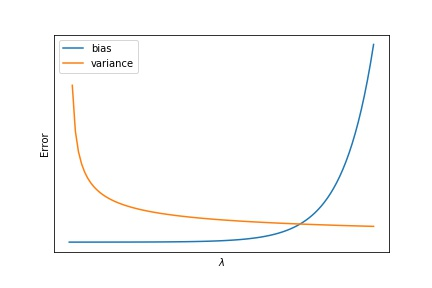
\includegraphics[width=0.5\paperwidth]{old/biasvariance_GEN.jpg}
    \caption{Bias and variance both contribute to the overall error of our model.}
    \label{fig:bias-vs-variance}
\end{figure}

For a moment, consider what happens on the far left side of this graph. Our variance is very high, and our bias is very low. In effect, we're fitting perfectly to all of the data in our dataset. This is exactly why we introduced the idea of regularization from before - we're fitting a very convoluted line that is able to pass through all of our data but which doesn't generalize well to new data points. There is a name for this: $\bm{overfitting}$.

\begin{definition}[overfitting]
    A phenomenon where we construct a convoluted model that is able to predict every point in our dataset perfectly but which doesn't generalize well to new data points.
\end{definition}

The opposite idea, $\bm{underfitting}$, is what happens at the far right of the graph: we have high bias and aren't responding to the variation in our dataset at all.

\begin{definition}[underfitting]
    A phenomenon where we construct a model that doesn't respond to variation in our data.
\end{definition}

So you can hopefully now see that the bias-variance tradeoff is important to managing the problem of overfitting and underfitting. Too much variance in our model and we'll overfit to our dataset. Too much bias and we won't account for the trends in our dataset at all.

In general, we would like to find a sweet spot of moderate bias and variance that produces minimal error. In the next section, we will explore how we find this sweet spot.

\subsection{Cross-Validation}
We've seen that in choosing a model, we incur error that can be described in terms of bias and variance. We've also seen that we can regulate the source of error through regularization, where heavier regularization increases the bias of our model. A natural question then is how do we know how much regularization to apply to achieve a good balance of bias and variance?

Another way to look at this is that we've traded the question of finding the optimal number of basis functions for finding the optimal value of the regularization parameter $\lambda$, which is often an easier problem in most contexts.

One very general technique for finding the sweet spot of our regularization parameter, other hyperparameters, or even for choosing among entirely different models is known as $\bm{cross-validation}$.

\begin{definition}[cross-validation]
    A subsampling procedure used over a dataset to tune hyperparameters and avoid over-fitting. Some portion of a dataset (10-20\% is common) is set aside, and training is performed on the remaining, larger portion of data. When training is complete, the smaller portion of data left out of training is used for testing. The larger portion of data is sometimes referred to as the \textit{training set}, and the smaller portion is sometimes referred to as the \textit{validation set}.
\end{definition}

Cross-validation is often performed more than once for a given setting of hyperparameters to avoid a skewed set of validation data being selected by chance. In $\bm{K-Folds cross-validation}$, you perform cross-validation $\bm{K}$ times, allocating $\frac{1}{\bm{K}}$ of your data for the validation set at each iteration.

Let's tie this back into finding a good regularization parameter. For a given value of $\lambda$, we will incur a certain amount of error in our model. We can measure this error using cross-validation, where we train our model on the training set and compute the final error using the validation set. To find the optimal value for $\lambda$, we perform cross-validation using different values of $\lambda$, eventually settling on the value that produces the lowest final error. This will effectively trade off bias and variance, finding the value of $\lambda$ that minimizes the total error.

You might wonder why we need to perform cross-validation at all - why can't we train on the entire dataset and then compute the error over the entire dataset as well?

The answer is again overfitting. If we train over the entire dataset and then validate our results on the exact same dataset, we are likely to choose a regularization parameter that encourages our model to conform to the exact variation in our dataset instead of finding the generalizable trends. By training on one set of data, and then validating on a completely different set of data, we force our model to find good generalizations in our dataset. This ultimately allows us to pick the regularization term $\lambda$ that finds the sweet spot between bias and variance, overfitting and underfitting.

\subsection{Making a Model Choice}
Now that we're aware of overfitting, underfitting, and how those concepts relate to the bias-variance tradeoff, we still need to come back to the question of how we actually select a model. Intuitively, we are trying to find the middle ground between bias and variance: picking a model that fits our data but that is also general enough to perform well on yet unseen data. Furthermore, there is no such thing as the `right' model choice. Instead, there are only model options that are either better or worse than others. To that end, it can be best to rely on the techniques presented above, specifically cross-validation, to make your model selection. Then, although you will not be able to make any sort of guarantee about your selection being the `best' of all possible models, you can at least have confidence your model achieved the best generalizability that could be proven through cross-validation.

\subsection{Bayesian Model Averaging}
We can also handle model selection using a Bayesian approach. This means we account for our uncertainty about the true model by averaging over the possible candidate models, weighting each model by our prior certainty that it is the one producing our data. If we have $M$ models indexed by $m = 1, ..., M$, we can write the likelihood of observing our dataset $\bm{X}$ as follows:
\begin{align*}
    p(\bm{X}) = \sum_{m=1}^{M} p(\bm{X}|m)p(m)
\end{align*}
where $p(m)$ is our prior certainty for a given model and $p(\bm{X}|m)$ is the likelihood of our dataset given that model. The elegance of this approach is that we don't have to pick any particular model, instead choosing to marginalize out our uncertainty.

\section{Linear Regression Extras}
With most of linear regression under our belt at this point, it's useful to drill down on a few concepts to come to a deeper understanding of how we can use them in the context of linear regression and beyond.

\subsection{Predictive Distribution}
Remaining in the setting of Bayesian Linear Regression, we may wish to get a distribution over our weights $\bm{w}$ instead of a point estimator for it using maximum likelihood. As we saw in Section \ref{bayesian-regularization-section}, we can introduce a prior distribution over $\bm{w}$, then together with our observed data, we can produce a posterior distribution over $\bm{w}$ as desired.

\begin{derivation}[posterior predictive derivation]
    For the sake of simplicity and ease of use, we will select our prior over $\bm{w}$ to be a Normal distribution with mean $\boldsymbol{\mu}_0$ and variance $\boldsymbol{S}_0^{-1}$:
    \begin{align*}
        p(\bm{w}) = \mathcal{N}(\boldsymbol{\mu}_0, \boldsymbol{S}_0^{-1})
    \end{align*}
    Remembering that the observed data is normally distributed, and accounting for Normal-Normal conjugacy, our posterior distribution will be Normal as well:
    \begin{align*}
        p(\bm{w}|\bm{X},\bm{y}, \beta) = \mathcal{N}(\boldsymbol{\mu}_n, \boldsymbol{S}_n^{-1})
    \end{align*}
    where
    \begin{align*}
        \boldsymbol{S}_n = (\boldsymbol{S}_0^{-1} + \beta\bm{X}\T\bm{X})^{-1} \\
        \boldsymbol{\mu}_n = \boldsymbol{S}_n(\boldsymbol{S}_0^{-1}\boldsymbol{\mu}_0 + \beta\bm{X}\bm{y})
    \end{align*}

    We now have a posterior distribution over $\bm{w}$. However, usually this distribution is not what we care about. We're actually interested in making a point prediction for the target $y^*$ given a new input $\bm{x}^*$. How do we go from a posterior distribution over $\bm{w}$ to this prediction? \\

    The answer is using what's known as the \textbf{posterior predictive} over $y^*$ given by:
    \begin{equation}
    \begin{split}
        p(y^* | \bm{x}^*, \bm{X}, \bm{y}) &= \int_{\bm{w}} p(y^* | \bm{x}^*, \bm{w})p(\bm{w} | \bm{X}, \bm{y})d\bm{w} \\
        &= \int_{\bm{w}} \mathcal{N}(y^* | \bm{w}\T\bm{x}^*, \beta^{-1})\mathcal{N}(\bm{w} | \boldsymbol{\mu}_n, \boldsymbol{S}_n^{-1})d\bm{w}
    \end{split}
    \end{equation}
\end{derivation}

\textbf{The idea here is to average the probability of $y^*$ over all the possible setting of $\bm{w}$, weighting the probabilities by how likely each setting of $\bm{w}$ is according to its posterior distribution.}

\section{Conclusion}
In this chapter, we looked at a specific tool for handling regression problems known as linear regression. We've seen linear regression described in terms of loss functions, probabilistic expressions, and geometric projections, which reflects the deep body of knowledge that we have around this very common technique.

We've also discussed many concepts in this chapter that will prove useful in other areas of machine learning, particularly for other supervised techniques: loss functions, regularization, bias and variance, over and underfitting, posterior distributions, maximum likelihood estimation, and cross-validation among others. Spending time to develop an understanding of these concepts now will pay off going forward.

It may or may not be obvious at this point that we are missing a technique for a very large class of problems: those where the solution is not just a continuous, real number. How do we handle situations where we need to make a choice between different discrete options? This is the question we will turn to in the next chapter.
